%- block legend
\begin{center}
    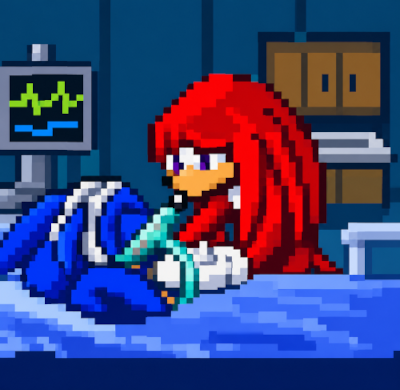
\includegraphics[scale=0.22]{duvida.png}
\end{center}

Após uma feroz batalha contra o malvado dr. Robotnik, Sonic ficou gravemente
ferido e foi internado no hospital de Mobius. Assim que soube da notícia, seu
amigo Knuckles foi lhe visitar.

Vendo o estado do herói, Knuckles resolveu que chegou a hora de tirar sua grande
dúvida:
``Sonic me diga... me diga onde fica o \texttt{h} em \texttt{corinthians}!''.
No que Sonic respondeu: ``\texttt{h} é a sétima letra de \texttt{corinthians},
portanto, fica na posição 7''.

Knuckles então resolveu tirar outra dúvida: ``E onde fica a letra $C$ na palavra
$P$?''. Mas desta vez, Sonic não teve forças para responder. Por isso, responda
você a grande dúvida de Knuckles.

%- endblock

%- block input
A primeira linha contém $C$, uma letra minúscula.\\
A segunda linha contém a palavra $P$ ($\VAR{N.min} \leq |P| \leq \VAR{N.max | sci}$), sem espaços e contendo apenas letras minúsculas.
%- endblock

%- block output
Imprima a posição da letra $C$ na palavra $P$. Se a letra aparecer em mais de
uma posição, imprima apenas a primeira em que aparece. Se a letra não aparecer em $P$, imprima
\texttt{-1} .
%- endblock

%- block editorial
Percorra todas as posições da palavra $P$,
testando se cada letra \texttt{P[i]} é igual a $C$, e parando assim que a primeira
posição de $C$ for encontrada. Se a letra não foi encontrada após o final do
laço, imprima \texttt{-1}.

Complexidade: $O(|P|)$

%- endblock
